\hypertarget{dsgvo-und-digitale-transformation}{%
\section{DSGVO und digitale
Transformation}\label{dsgvo-und-digitale-transformation}}

\hypertarget{lernziele}{%
\subsection{Lernziele}\label{lernziele}}

\begin{itemize}
\tightlist
\item
  Sie können selbständig entscheiden, ob für ein Schweizer
\item
  Unternehmen die DSGVO anwendbar ist oder nicht.
\item
  Sie kennen die notwendigen Schritte bei DSGVO-Projekten
\item
  Sie verstehen die Faktoren für die exponentielle Entwicklung der
  "Digitalen Transformation``
\item
  Sie kennen die Hype-Cycles
\item
  Sie kennen Rechtsaspekte bei der Digitalisierung von
  Geschäftsprozessen
\end{itemize}

\hypertarget{wann-dsgvo}{%
\subsection{Wann DSGVO?}\label{wann-dsgvo}}

Die DSGVO ist seit Ende Mai 2018 auch für Schweizer Unternehmen direkt
anwendbar, wenn: - diese \emph{Waren oder Dienstleistungen in der EU/EWR
anbieten} (die Angabe des Preises in Euro genügt) und \textbf{dazu
personenbezogene Daten} (z.B. Adressdaten, Kundenprofil) bearbeiten
(Marktortprinzip: Art. 3 Abs. 2 DSGVO) - diese das Verhalten von
\textbf{Website-Besuchern aus der EU sammeln} und auswerten (Tracking
durch Cookies, Profiling mit Tools wie Google Analytics, Facebook Pixel
etc.) - diese regelmässig \textbf{Newsletter} an Empfänger in der EU
versendet - diese im Auftrag oder als Konzernzentrale resp. -Mitglied
eines in der EU domizilierten Unternehmens personenbezogene Daten
bearbeiten

Das DSGVO ist nur ein Mindeststandard um ein eruopäisch
vereinheitlichtes Datenschutzrecht zur Durchsetzung von merheitlich
bereits bestehenden Grundsätzen. Die einzelnen Mitgliedsstaaten können
weitergehende Regelungen erfassen.

\hypertarget{rechte-in-der-dsgvo}{%
\subsection{Rechte in der DSGVO}\label{rechte-in-der-dsgvo}}

\begin{itemize}
\tightlist
\item
  \textbf{Auskunftsrecht} und \textbf{Recht auf Datenübertragbarkeit}
\item
  \textbf{Erweiterte Informationspflichten} gegenüber der betroffenen
  Person
\item
  \textbf{Widerspruchsrecht}
\item
  \textbf{Recht auf Löschung} (Recht auf Vergessen)
\item
  Möglichkeit für \textbf{Abmahnungen} und Klagen von
  \textbf{Genugtuung} und \textbf{Schadenersatz} für die betroffene
  Person
\item
  \textbf{Privacy by design} und \textbf{privacy by default} (!)
\item
  Erweiterte \textbf{Dokumentationspflichten} (TOM's,
  Verarbeitungsverzeichnisse, Beweislastumkehr)
\end{itemize}

\hypertarget{toms}{%
\subsubsection{TOM's}\label{toms}}

Es muss dokumentiert werden, wie die informationstechnischen
Gerätschafte aufgestellt sind und wer verantwortlich ist.

\hypertarget{was-ist-zu-tun}{%
\subsection{Was ist zu tun?}\label{was-ist-zu-tun}}

\begin{figure}
\centering
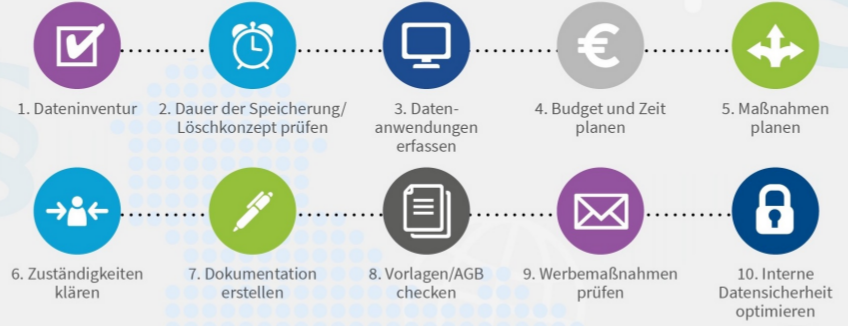
\includegraphics{figures/dsgvoSteps.png}
\caption{Steps DSGVO}
\end{figure}

\textbf{Grundlage jedes Datenschutz-Audits ist die Erhebung des
aktuellen Zustandes}:\\
Welche personenbezogenen Daten sind vorhanden? In welcher Form und wo?
Zu welchem Zweck? Wer zeichnet sich verantwortlich? Wer hat Zugang? Wie
lange werden diese gespeichert? Handelt es sich um besonders
schützenswerte Personendaten? Wie werden diese technisch \&
organisatorisch geschützt? Wie wird das Risiko einer Verletzung \& deren
Folgen beurteilt?
